\documentclass{article}


% if you need to pass options to natbib, use, e.g.:
%     \PassOptionsToPackage{numbers, compress}{natbib}
% before loading neurips_2023


% ready for submission
% \usepackage{neurips_2023}


% to compile a preprint version, e.g., for submission to arXiv, add add the
% [preprint] option:
  \usepackage[preprint]{neurips_2023}


% to compile a camera-ready version, add the [final] option, e.g.:
  % \usepackage[final]{neurips_2023}


% to avoid loading the natbib package, add option nonatbib:
  %  \usepackage[nonatbib]{neurips_2023}


\usepackage[utf8]{inputenc} % allow utf-8 input
\usepackage[T1]{fontenc}    % use 8-bit T1 fonts
\usepackage{hyperref}       % hyperlinks
\usepackage{url}            % simple URL typesetting
\usepackage{booktabs}       % professional-quality tables
\usepackage{amsfonts}       % blackboard math symbols
\usepackage{nicefrac}       % compact symbols for 1/2, etc.
\usepackage{microtype}      % microtypography
\usepackage{xcolor}         % colors
\usepackage{graphicx}       % Required for including graphics
\usepackage{subcaption}     % Required for subfigure environment
\usepackage{listings}       % Required for lstlisting environment
\usepackage{float}          % Enables tables to be rendered anywhere on the page
\usepackage{amsmath}        % For math environments like equation
\usepackage{pgfplots}       % For histogram
\usepackage{tikz}           % For histogram
\pgfplotsset{compat=1.18}


\title{BME1312 Project1 Report: Deep Learning for MRI Reconstruction}


% The \author macro works with any number of authors. There are two commands
% used to separate the names and addresses of multiple authors: \And and \AND.
%
% Using \And between authors leaves it to LaTeX to determine where to break the
% lines. Using \AND forces a line break at that point. So, if LaTeX puts 3 of 4
% authors names on the first line, and the last on the second line, try using
% \AND instead of \And before the third author name.


\author{%
  Wenye Xiong \\
  2023533141 \\
  \texttt{xiongwy2023@shanghaitech.edu.cn}
  \And
  Renyi Yang \\
  2023533030 \\
  \texttt{yangry2023@shanghaitech.edu.cn}
  \AND
  Jiaxing Wu \\
  2023533160 \\
  \texttt{wujx2023@shanghaitech.edu.cn}
  \And
  Boyang Xia \\
  2023533073 \\
  \texttt{xiaby2023@shanghaitech.edu.cn}
  \AND
  Fengmin Yang \\
  2023533183 \\
  \texttt{yangfm2023@shanghaitech.edu.cn}
}

\begin{document}


\maketitle


\begin{abstract}
This report details the implementation and evaluation of U-Net based deep learning models for cardiac segmentation 
in cine MRI scans. The project focuses on segmenting three key structures: the Left Ventricle (LV), Right Ventricle (RV), 
and Myocardium (MYO). We explore the standard U-Net architecture, the impact of removing skip connections, the effect of 
data augmentation, and the performance difference between Binary Cross-Entropy (BCE) loss and Soft Dice loss.
\end{abstract}

\section{Introduction}
This project aims to:
\begin{enumerate}
    \item Implement a U-Net model for segmenting LV, RV, and MYO from cardiac cine MRI images.
    \item Investigate the role of skip connections in the U-Net architecture.
    \item Evaluate the impact of data augmentation on segmentation performance.
    \item Compare Binary Cross-Entropy loss with Soft Dice loss for training the segmentation model.
\end{enumerate}



\section{Baseline U-Net}

\subsection{Network}
The U-Net architecture consists of:
\begin{itemize}
    \item \texttt{DoubleConv}: A block of two sequential (Conv2D 3x3, BatchNorm2D, ReLU) operations.
    \item \texttt{Down}: Max pooling (2x2) followed by a \texttt{DoubleConv} block for downsampling in the encoder.
    \item \texttt{Up}: Upsampling (bilinear or transpose convolution) followed by concatenation with features from the 
    corresponding encoder layer (skip connection) and a \texttt{DoubleConv} block. Padding is used to handle potential 
    size mismatches during concatenation.
\end{itemize}

Our baseline is as below:
\begin{itemize}
    \item \textbf{Network}: The standard \texttt{UNet} class as described above, with \texttt{C\_base=32}, 1 input channel, 
    and 3 output classes. Bilinear upsampling was used.
    \item \textbf{Loss Function}: A custom \texttt{MyBinaryCrossEntropy} loss was used. This involves applying a Sigmoid 
    function to the model's output logits to get probabilities, then computing \texttt{nn.BCELoss} against the 3-channel 
    binary ground truth masks. The learning rate was 0.01.
    \item \textbf{Evaluation}: Mean and standard deviation of the Dice Similarity Coefficient (DSC) for LV, RV, and MYO 
    were calculated on the test set. Training and validation loss curves were plotted by the solver. 
    Example segmentation results were saved.
\end{itemize}

\subsection{Experiments and Results}
The training loss and validation loss of the baseline U-Net are shown in figure \ref{fig:baseline_unet_loss}
\begin{figure}[H]
  \centering
  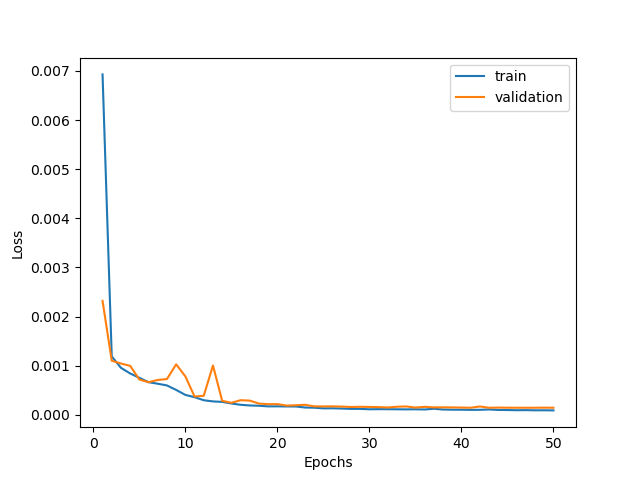
\includegraphics[width=\linewidth]{../result/baseline_unet.png}
  \caption{Training and Validation Loss Curves for the Baseline UNet}
  \label{fig:baseline_unet_loss}
\end{figure}

And here is an example segmentation result in figure \ref{fig:baseline_unet_segmentation_example}
\begin{figure}[H]
  \centering
  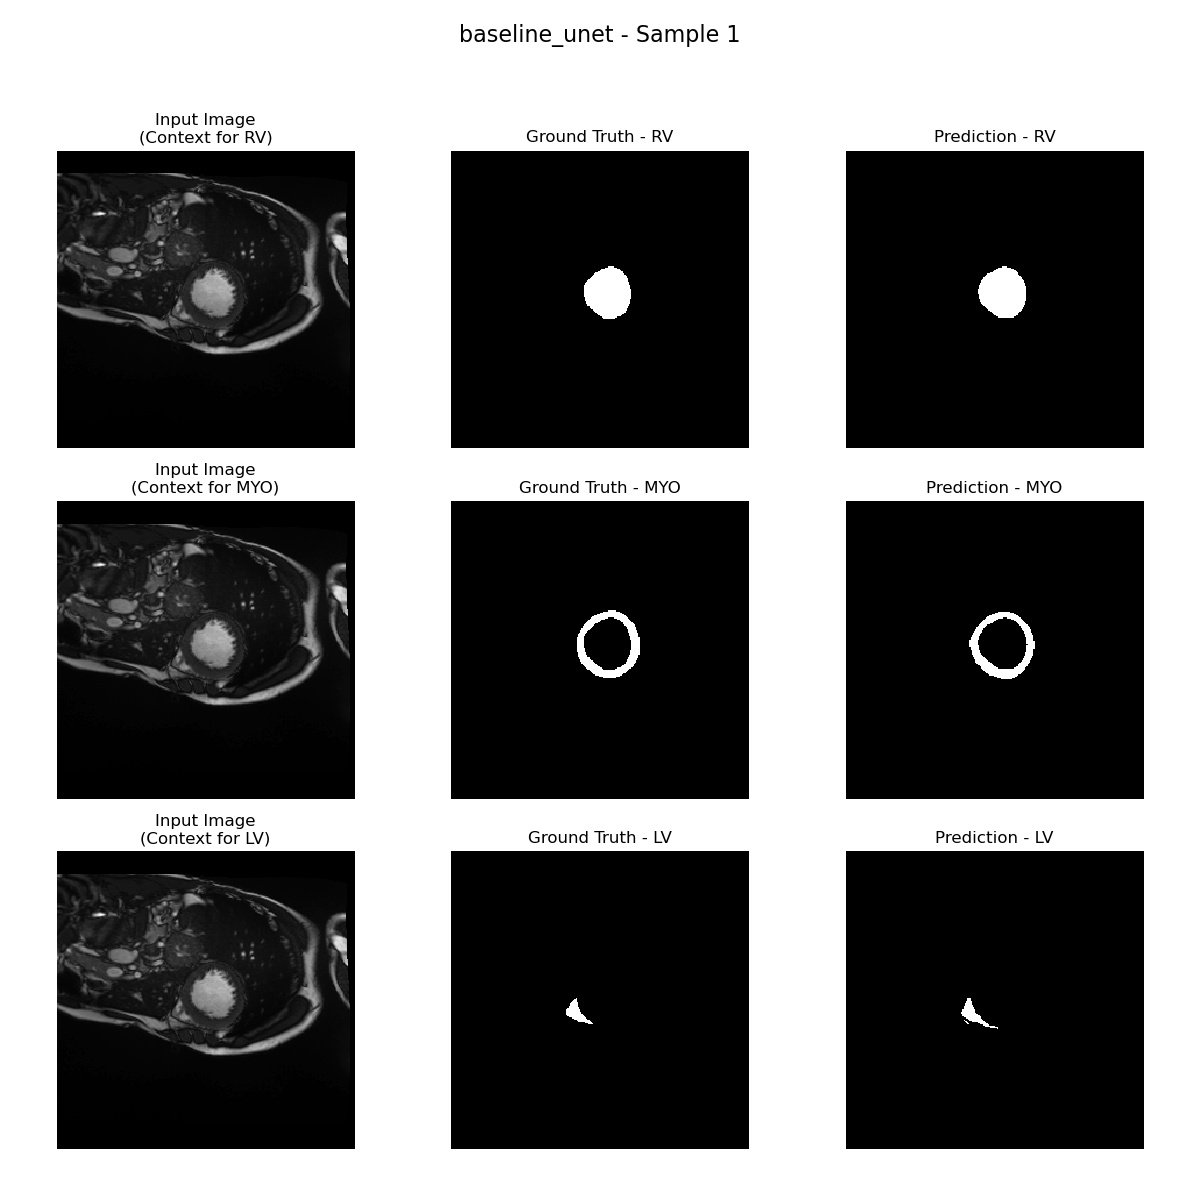
\includegraphics[width=\linewidth]{../result/baseline_unet/sample_1_segmentation.png}
  \caption{An Example Segmentation for the Baseline UNet}
  \label{fig:baseline_unet_segmentation_example}
\end{figure}

The baseline U-Net trained with Binary Cross-Entropy loss achieved the following Dice scores:
\begin{table}[H]
\centering
\caption{Dice Coefficients for Baseline U-Net (Task a)}
\label{tab:baseline_unet}
\begin{tabular}{lcc}
\toprule
Structure & Mean Dice & Standard Deviation \\
\midrule
RV        & 0.9498    & 0.0089             \\
MYO       & 0.8755    & 0.0120             \\
LV        & 0.8960    & 0.0361             \\
\bottomrule
\end{tabular}
\end{table}

\subsection{Discussion}
The baseline U-Net (Table \ref{tab:baseline_unet}) demonstrated strong segmentation performance.
\begin{itemize}
    \item \textbf{RV Segmentation}: Achieved the highest mean Dice score (0.9498). This is often expected as the RV is 
    typically a large, relatively well-defined structure with good contrast against surrounding tissues in many MRI sequences.
    \item \textbf{LV Segmentation}: Also showed good performance with a mean Dice of 0.8960. The LV cavity is usually clearly visible.
    \item \textbf{MYO Segmentation}: Had the lowest mean Dice score (0.8755). The myocardium is a thinner, more complex structure 
    surrounding the LV, and its boundaries, especially with the LV cavity (endocardium) and epicardium, can be more challenging to 
    delineate accurately, potentially leading to lower overlap scores.
\end{itemize}
The standard deviations are relatively small, indicating consistent performance across the test slices. Overall, the baseline U-Net 
provides a solid foundation for cardiac segmentation.












% \begin{figure}[H]    放图片
%   \centering
%   \includegraphics[width=\linewidth]{../assets/Training Loss and Validation Loss Unrolled.png}
%   \caption{Training and Validation Loss Curves for the 3-Cascade Unrolled Network}
%   \label{fig:loss_unrolled}
% \end{figure}


% \begin{figure}[H]  直方图
%   \centering
%   \begin{tikzpicture}
%     \begin{axis}
%     [ybar, 
%     grid = major, major grid style = {dashed},
%     ymin = 0,
%     ylabel = {SSIM values},
%     title = {SSIM Values for Each Model},
%     bar width = .5cm,
%     width = 40cm,
%     height = 6cm,
%     symbolic x coords={M1, M2, M3, U1, U2, U3},
%     x = 2cm,
%     xtick = data,
%     nodes near coords,
%     nodes near coords style = {font = \fontsize{8}{12}\selectfont},
%     enlarge x limits = 0.2,
%     legend style = {at = {(0.5,-0.2)},anchor = north,legend columns = -1},
%     ] 
%     \addplot+ coordinates {(M1, 0.743) (M2, 0.844) (M3, 0.844) (U1, 0.834) (U2, 0.815) (U3, 0.807)}; 
%     \addplot+ coordinates {(M1, 0.037) (M2, 0.037) (M3, 0.042) (U1, 0.030) (U2, 0.037) (U3, 0.041)}; 
%     \legend{SSIM mean, SSIM std};
%     \end{axis} 
%   \end{tikzpicture}
%   \caption{SSIM Values for Each Model}
%   \label{fig:SSIM Values for Each Model}
% \end{figure}



\end{document}